\documentclass{article}
\usepackage{amsmath, sfmath, multicol, tkz-euclide, array, enumerate, tcolorbox, tabularray}
\renewcommand{\familydefault}{\sfdefault}
\setlength{\parindent}{0cm}
\pagestyle{empty}
\usepackage[left=1in, top=0.5in, right=1in, bottom=0.5in]{geometry}
\tikzset{>=stealth}
\tcbset{colback=white}

\newcounter{example}[section]
\newenvironment{example}[1][]{\refstepcounter{example}\par\medskip
   {\color{red}\textbf{Example~\theexample. #1}}}{\medskip}

\begin{document}

\section*{Isosceles and Equilateral Triangles}

\begin{tcolorbox}[colframe=orange!70!white, coltitle=black, title=\textbf{Today I Can}]
\begin{enumerate}
    \item Use and apply properties of isosceles and equilateral triangles.
\end{enumerate}
\end{tcolorbox}

\subsection*{Isosceles Triangles}

\begin{center}
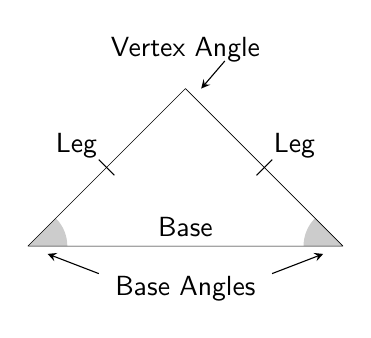
\begin{tikzpicture}
\tkzDefPoints{0/0/A, 4/0/B, 2/2/C}
\tkzLabelSegment[below, yshift=-0.1in](A,B){Base Angles}
\tkzLabelSegment[above](A,B){Base}
\tkzMarkSegments[mark=|](B,C A,C)
\tkzLabelSegment[above left](A,C){Leg}
\tkzLabelSegment[above right](B,C){Leg}
\tkzLabelAngle[pos=-0.5](A,C,B){Vertex Angle}
\tkzFillAngle[size = 0.5, color=gray!40](B,A,C)
\tkzFillAngle[size=0.5, color=gray!40](C,B,A)
\tkzDrawPolygon(A,B,C)
\draw [->, >=stealth] (2.5,2.35) --  (2.2,2);
\draw [->, >=stealth] (0.9,-0.35) -- (0.25,-0.1);
\draw [->, >=stealth] (3.1,-0.35) -- (3.75, -0.1);
\end{tikzpicture}
\end{center}

\begin{tcolorbox}[colframe=black!20!white, opacitybacktitle=0.1, coltitle=black, title=\textbf{Base Angle Theorem}]
If 2 sides of a triangle are congruent, then the angles across from those sides are congruent.
\newline

\begin{center}
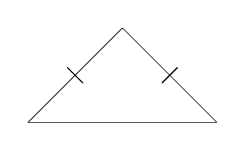
\begin{tikzpicture}[scale=0.6]
\tkzDefPoints{0/0/A, 4/0/B, 2/2/C}
\tkzMarkSegments[mark=|](B,C A,C)
\tkzDrawPolygon(A,B,C)
\end{tikzpicture}
\hspace{0.25in}
\raisebox{0.5cm}{$\implies$}
\hspace{0.25in}
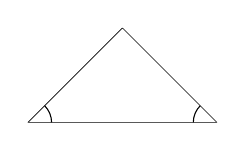
\begin{tikzpicture}[scale=0.6]
\tkzDefPoints{0/0/A, 4/0/B, 2/2/C}
\tkzDrawPolygon(A,B,C)
\tkzMarkAngles[size = 0.5](B,A,C C,B,A)
\end{tikzpicture}
\end{center}
\end{tcolorbox}

\begin{tcolorbox}[colframe=black!20!white, opacitybacktitle=0.1, coltitle=black, title=\textbf{Base Angle Converse}]
If 2 angles of a triangle are congruent, then the sides across from those angles are congruent.
\newline

\begin{center}
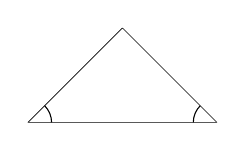
\begin{tikzpicture}[scale=0.6]
\tkzDefPoints{0/0/A, 4/0/B, 2/2/C}
\tkzDrawPolygon(A,B,C)
\tkzMarkAngles[size = 0.5](B,A,C C,B,A)
\end{tikzpicture}
\hspace{0.25in}
\raisebox{0.5cm}{$\implies$}
\hspace{0.25in}
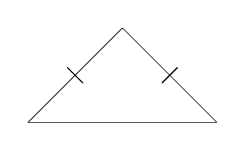
\begin{tikzpicture}[scale=0.6]
\tkzDefPoints{0/0/A, 4/0/B, 2/2/C}
\tkzMarkSegments[mark=|](B,C A,C)
\tkzDrawPolygon(A,B,C)
\end{tikzpicture}
\end{center}
\end{tcolorbox}

% \begin{example}
% Use the diagram to answer each. 
% \begin{center}
% \begin{tikzpicture}[scale=0.7]
% \tkzDefPoints{0/0/A, 4/0/C, 2/4/B, 2/0/E, 1/2/D}
% \tkzDrawPolygon(A,B,C)
% \tkzDrawSegment(D,E)
% \tkzLabelPoints[left](A,D,B)
% \tkzLabelPoints[below](E,C)
% \tkzMarkAngles[size=0.5](B,C,A C,A,B)
% \tkzMarkSegments[mark=|](A,D D,E)
% \end{tikzpicture}
% \end{center}
% \smallskip 
% \begin{multicols}{2}
% \begin{enumerate}[(a)]
%     \item Is $\overline{AB} \cong \overline{CB}$? Explain.
%     \item Is $\angle A \cong \angle DEA$? Explain.
% \end{enumerate}
% \end{multicols}
% \end{example}

\begin{example}
Find the value of $x$ in each.
\begin{multicols}{2}
\begin{enumerate}[(a)]
    \item \mbox{} \newline 

    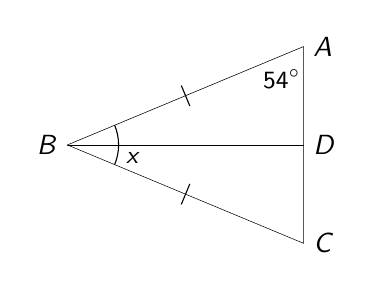
\begin{tikzpicture}[baseline=0pt]
    \tkzDefPoints{0/0/B, 3/0/D, 3/1.25/A, 3/-1.25/C}
    \tkzDrawPolygon(A,B,C)
    \tkzDrawSegment(B,D)
    \tkzMarkSegments[mark=|](A,B C,B)
    \tkzMarkAngles[size=0.65](D,B,A C,B,D)
    \tkzLabelPoints[left](B)
    \tkzLabelPoints[right](A,D,C)
    \tkzLabelAngle[pos=0.5](B,A,D){\small $54^\circ$}
    \tkzLabelAngle[pos=0.85](C,B,D){\small $x$}
    \end{tikzpicture}

    \item \mbox{} \newline 

    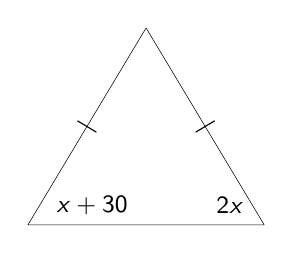
\begin{tikzpicture}[baseline=0pt]
    \tkzDefPoints{0/0/A, 3/0/B, 1.5/2.5/C}
    \tkzDrawPolygon(A,B,C)
    \tkzMarkSegments[mark=|](A,C B,C)
    \tkzLabelAngle[pos=0.5, xshift=0.15in](B,A,C){\small $x+30$}
    \tkzLabelAngle[pos=0.5](C,B,A){\small $2x$}
    \end{tikzpicture}
\end{enumerate}
\end{multicols}
\end{example}

\newpage 

\begin{tcolorbox}[colframe=black!20!white, opacitybacktitle=0.1, coltitle=black, title=\textbf{Corollary}]
A \textbf{corollary} is a theorem that can be easily proven using another theorem.
\end{tcolorbox}

\smallskip 

\begin{itemize}
    \item Corollary to Base Angle Theorem:
    \begin{itemize}
        \item If a triangle is equilateral then each angle is congruent.
    \end{itemize}
    \item Corollary to Base Angle Converse:
    \begin{itemize}
        \item If the 3 angles of a triangle are congruent, then the triangle is equilateral.
    \end{itemize}
\end{itemize}

\subsection*{Equilateral Triangles}

\begin{example}
The measures of two sides of an equilateral triangle are $3x+15$ and $7x-5$. 
\vspace{2.5in}
\begin{enumerate}[(a)]
    \item What is the measure of the 3rd side?  \vspace{1.5in}
    \item Find the perimeter of the triangle.   \vspace{1.5in}
    \item What is the measure of each angle? 
\end{enumerate}
\end{example}

\end{document}
